\chapter{Routing}

Routing determine the ``good''\footnote{The minimum path typically} path (
sequence of routers) thru network from source to destination.
Routing protocols use graphs as a mathematical abstraction.

\section{Typologies of routing}

Routing can be \textbf{global}, \textbf{decentralized}, \textbf{static} (where
the route change slowly over time) and \textbf{dynamic} (where the routes change
quickly over time).

\subsection{Global routing}

In this kind of routing routers have the complete topology of the network, with
information about links cost.
Characteristics:
\begin{itemize}
\item ``link state'' algorithm
\item efficent but not faseable
\end{itemize}

An example of a global routing algorithm is the one made by Dijkstra.

\subsubsection{Dijkstra's algorithm}

In this algorithm, that's iterative, all the nodes know link cost between each
other. Basically, it computes least cost path from one note to all the others.

\begin{figure}[t]
  \captionsetup{singlelinecheck=off}
  \centering
  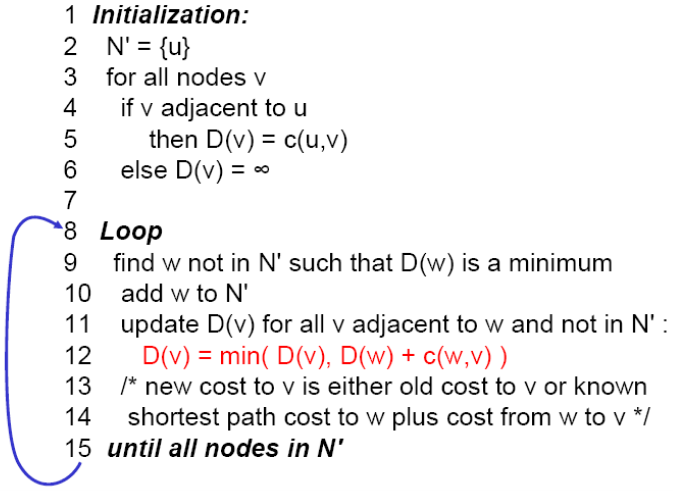
\includegraphics[scale=0.45]{DijkstraAlgo}
  \caption[Dijkstra's algorithm]{Dijkstra's algorithm. Notation:
    \begin{itemize}
    \item $c(x, y)$: link cost from node $x$ to $y$. It's $\infty$ if not direct
      neighbors
    \item $D(v)$: current value of cost of path from source to destination $v$
    \item $p(v)$: predecessor node along path from source to $v$
    \item $N'$: set of nodes whose least cost path definitively known
    \end{itemize}
  }
\end{figure}

\subsection{Decentralized routing}
In this type of routing routers know physically-connected neighbors, and link
cost to them. There is a iterative process of computation and exchange of
information with neighbors.
This algorithms are defined as ``distance vector'' algorithms.

\subsection{Routing based on network typology}

There are different types of routing based on different types of networks.

\paragraph*{Infrastructure based} In this case routing is relatively simple.
There is just a simgle hop from the access point (AP) to the wireless node.

\paragraph*{MANET} Also know as ad-hoc, it has the following characteristics:
\begin{itemize}
\item the network costantly changes
\item wireless nodes are not necessarily all adjacent, so data forwarding
  could be necessary
\end{itemize}
Additionally, there are other difficulties, such as energy consumption and
limited bandwidth (due exchange of routing information) on mobile systems. In
wireline networks we have symmetric links, limited redundancy and fixed
typology, insteas in wireless has asymmetric links, random redundancy with
unplanned, dynamic links. With all this pecurialities, traditional routing
algorithms for MANETS\footnote{MANET stands for \textit{Metropolitan Area
    Network}} are inefficent, and the new one must rely on data link
information, not just network layer updates\footnote{Layer updates only
  determine connectivity}, without using in centralized approaches because they
just don't work. In MANETS nodes can be routers, and they can send different
type of messages between them.
\subparagraph*{Messages classification} There are different type of messages:
\begin{itemize}
\item Unicast: trasmission 1 to 1. In order to achieve a good unicast routing
  protocol there are some goals:
  \begin{itemize}
  \item minimal control overhead
  \item multi-hop path routing capability
  \item no loops
  \end{itemize}
\item Multicast: transmission 1 to N: different receivers of the same message,
  that it can follow different paths
\item Broadcast: transmission 1 to N: everyone receives the message
\end{itemize}

\section{Protocols classification}

\begin{figure}[t]
  \centering
  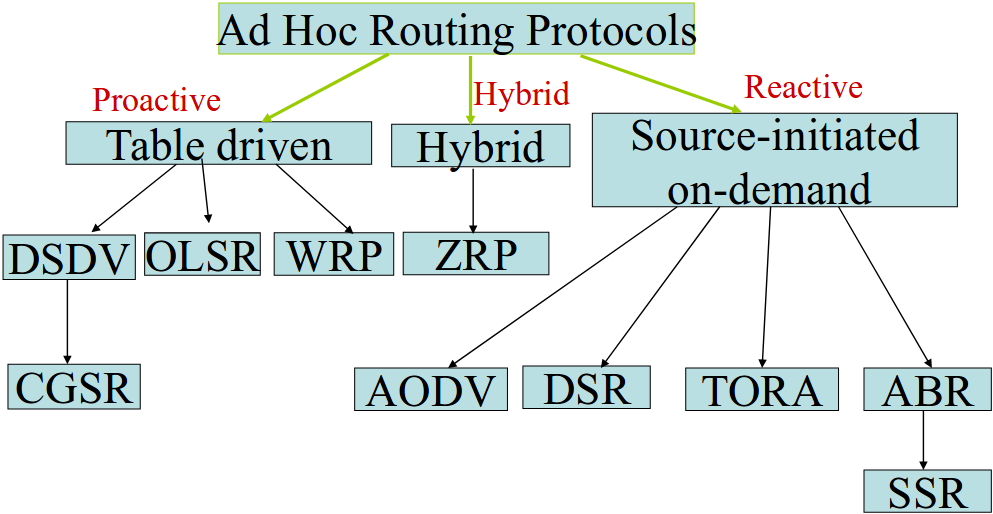
\includegraphics[scale=0.3]{AdHocRoutingProtocols}
  \caption{Tree listing all the ad-hoc routing protocols}
  \label{fig:mac:adHocRoutingProtocols}
\end{figure}

As shown in Figure~\ref{fig:mac:adHocRoutingProtocols} protocols can be
proactive or reactive, and are classificated as:
\begin{itemize}
\item table-driven (proactive) $\to$ up-to-date routing information are
  maintained
\item source-initiated (on demand/demand driven) $\to$ only routes in use are
  maintained
\item hybrid protocols $\to$ combination of proactive and reactive protocols
\end{itemize}

\subsection{Proactive protocols}

Proactive protocols are based on traditional distance-vector and link-state
protocols, where each node maintains a route to the other edge of the network.
This cause a high overhead in most scenarios, but since each node maintains and
updates its routing table, there is a low packet forwarding latency.

Due the proactive nature, changes to the network topology are immediately
propagated to all the nodes.

There are different typologies, that will be described below.

\subsubsection{DSDV (Destination Sequenced Distance Vector)}

Based on Bellum-Ford algorithm it has characteristics similar to Dijkstra's
algorithm, but with slower performace and a better versatility (it supports
negative weights). With DSDV, every route has a sequence number and packets are
transmitted according to the routing table: each node has a routing table with
all the nodes listed, and each node has its own sequence number.
The routing table consistency is kept trasmitting periodically updates and when
two routes to a destination is received from two different neightbors the one
with the gratest destination dequence number is choosen, otherwise the smallest
leap-count is kept % TODO check this part
Continuously updating the routing table can generate a lot of overhead, and
there are two ways to carry updates:
\begin{itemize}
\item performing a full dump
\item having incremental updates
\end{itemize}

\subsubsection{OLSR (optimized link state routing)}

This is based on the link state algorithm. It minimizes flooding of broadcasting
packets by using only the selected \textit{Multipoint Hop (MH)} called
\textit{Multipoint relays (MR)}. All links with neighboring MHs are declared and
are flooded in the entire network. MR minimize the flooding by reducing
duplicate retrasmission.

In general, OLSR is good for large and dense networks.

\subsubsection{CGSR}

In this typology, nodes are organized into a hierarchy of clusters: every
cluster has a \textit{cluster master (clusterhead)} that forward packets from
the other sets node.

\subsection{Reactive protocols}
The source builds routing on demand with a ``flooding'' method, but maintains
only active routes.
Advantages:
\begin{itemize}
\item less overhead
\item better scaling properties
\item route acquisition latency
\end{itemize}

Source-initiated on-demand routing protocols have the following characteristics:
\begin{itemize}
\item route created only when needed
\item flooding is used in order to find routes
\item router maintenance procedure is used to repair broken routes
\end{itemize}

\subsubsection{AODV (Ad hoc On-Demand Distance Vector Routing)}

This routing protocol, based on DSDV, exchange the routing table only along a
given route. In order to discover routes, there is a specific package, RREQ
(\textit{Route Request Packet}). The packet is sent from the sender to the
receiver, and when it's received, it's pinged back to the source, creating a
path.\todo{Is an RREP or an RREQ that is sent back? Need to be checked!}

Routes are timed: after a while they expire: unicast and multicast routes are
kept until a timeout happens.

\paragraph*{Properties} AODV's properties:
\begin{itemize}
\item discovers routes as and where necessary
\item routes are maintained just as long as necessary
\item sequence number gets increased every time the node notices chenges in the neightborhood topology
\end{itemize}

\paragraph*{How a package is sent} AODV use the following procedure to send a
packet:
\begin{enumerate}
\item routing table check to determine if the current route to destination is
  present. If so, forward the packet to the next hop, otherwise, go to step 2
\item begin discovery process with an RREQ\todo{Split the listing in
  two columns} \footnote{
  This packet is initially sent with a small time-to-live (TTL), to limit its
  propagation and avoid an eccessive flooding.
  The packet contains:
  \begin{itemize}
  \item source node's IP address
  \item source node's current sequence number
  \item destination IP address
  \item destination sequence number
  \end{itemize}
}
\item once an intermediate node receives a RREQ, the node sets up a reverse
  route entry for the source node in its route table
\item when RREQ reaches destination in order to responde to RREQ a node should
  have it in its route table (the route has to be unexpired). If conditions are
  true the node responds to RREQ by sending a RREP back using unicasting
  and not flooding to the source (using reverse path), otherwise the hop count
  is incremented and the packet broadcasted to its neighbors. Eventually, the
  RREQ will be able to reach the destination. Intermediate nodes can send an
  RREQ if they know a more recent path of the one previously known to senders.
\end{enumerate}

\paragraph*{Broadcast} The broadcast is performed by flooding the network, and
a sequence number on the packets is used to stop loops from happening, meaning
that a package could expire without have reached the destination. To solve this
problem, the life of a packet can be aumented, changing its time-to-live (TTL).
Using the flooding to broadcast packets has the following pros:
\begin{itemize}
\item simplicity
\item efficent when overhead for route discovery is higher than the data
  transfered
  \item potential higher reliability of data delivery
\end{itemize}
...but it has some cons too:
\begin{itemize}
\item very high overhead potentially
\item possibility of collision during packet propagation
\end{itemize}

\subsubsection{DSR (Dynamic Source Routing)}

With this ad-hoc routing protocol nodes maintains route caches, and the full
source-route is aggregated in RREQ and sent back in RREP. Each data packet has
full source route, casuing a little overhead increment.
Route discovery starts when the sender initiates requests and intermediate nodes
add their address onto request so that when the packet reaches destination it
contains all the full path.

\paragraph*{Differences with AODV} Being similar to AODV, it has the following
differences:
\begin{itemize}
\item DSR includes source routes, having large headers (and suffering degraded
  performances)
\item AODV keeps routing tables temporarily
\item AODV keeps routes only between nodes which need to comunicate with
\item DSR route cached entries don't expire
\end{itemize}

\section{Other routing \& metrics}

\subsection{Routing protocols}

\paragraph*{Signal stability routing} Here, the signal strengh is used as
metric, in combination with a DSR-like routing. RREQ is forwarded only if the
packet is received over a link with good signal strengh.

\paragraph*{Geographic routing protocols} This protocols use location. In
paricular, GPSR (greedy perimeter stateless routing) has the following
properties:
\begin{itemize}
\item location of the destination node is assumed to be known
\item each node knows location of its neightbors $\to$ packets are forwarded to
  the closest one
\item if there is a ``hole'' in the graph, use perimeter routing (right-hand rule) \todo{Maybe this role could be explained a little bit.}
\end{itemize}

\subsection{Metrics}

\paragraph*{Associativity-based} \todo{This part is confused, check this out!}
Defines metric with a ``dregree of association stability'' (with how many
frequency do I move from my neightboor?). Nodes with less mobility or better
links have higher stability volume.

\paragraph*{Exprected Transmission Time (ETT)} This metric is easier to computer
than the singnal strengh, and it can be more useful.

\paragraph*{Weighted cumulative expected transmission time} This metric is
better for multi-radio and asymmetric route links.
